\RequirePackage{luatex85}
\documentclass[tikz, border=10pt]{standalone}

\usepackage[compat=1.1.0]{tikz-feynman}

\begin{document}

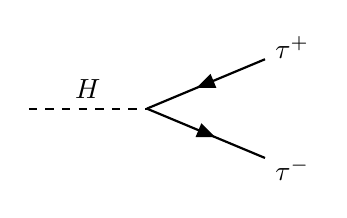
\begin{tikzpicture}[thick]
 \begin{feynman}
  \vertex (origin);
  \vertex [right=1.5cm of origin] (H);
  \vertex [above right=0.50cm and 1.5cm of H] (tau1) {\(\tau^{+}\)};
  \vertex [below right=0.50cm and 1.5cm of H] (tau2) {\(\tau^{-}\)};
  \diagram* {
  (origin) -- [scalar, edge label={\(H\)}] (H),
  (tau1) -- [fermion] (H) -- [fermion] (tau2),
  };
 \end{feynman}
\end{tikzpicture}
\end{document}
